\documentclass[a4paper,12pt,twocolumn]{article}

\usepackage[utf8]{inputenc}
\usepackage[T1]{fontenc}
\usepackage{fullpage}
\usepackage{graphicx}
\usepackage{url}
\usepackage{xspace}
\usepackage[francais]{babel}
\usepackage{appendix}
\usepackage[bmargin=2cm,tmargin=2cm,lmargin=2cm,rmargin=2cm]{geometry}
\usepackage{color}
\usepackage{listings}
\lstset{
  morekeywords={abort,abs,accept,access,all,and,array,at,begin,body,
      case,constant,declare,delay,delta,digits,do,else,elsif,end,entry,
      exception,exit,for,function,generic,goto,if,in,is,limited,loop,
      mod,new,not,null,of,or,others,out,package,pragma,private,
      procedure,raise,range,record,rem,renames,return,reverse,select,
      separate,subtype,task,terminate,then,type,use,when,while,with,
      xor,abstract,aliased,protected,requeue,tagged,until},
  sensitive=f,
  morecomment=[l]--,
  morestring=[d]",
  showstringspaces=false,
  basicstyle=\small\ttfamily,
  keywordstyle=\bf\small,
  commentstyle=\itshape,
  stringstyle=\sf,
  extendedchars=true,
  columns=[c]fixed
}

\usepackage{fancyhdr}

\pagestyle{fancyplain}
\lhead{\footnotesize\sf CPSC 565 - Winter 2013}
\rhead{\footnotesize\sf Cédric Guillot}

\title{Chess AI improvement through an evolutionary approach}
\author{Cédric Guillot, University of Calgary (cpguillo@ucalgary.ca)}
\date{April 30, 2013}

\begin{document}

\maketitle

\begin{abstract}
This paper presents the results in the attempt of improving a classic chess AI by using an evolutionary approach. The general idea is to fine-tune the parameters used by the chess AI (pieces values) in its board evaluation.
\end{abstract}

\section{Introduction and Goals}
Chess AI has been a subject of interest for over 70 years now. The first paper program that could play a game of chess was written in 1951 by Alan turing, and the most symbolic achievement was Deep Blue (chess AI developed by IBM) that beated the former world champion Garry Kasparov in a regular cheess match.\\
Strategies for chess AI have improved but they still use parameters assigned to each kind of pieces in order to evaluate how favorable the chess board currently is to us. For that reason, this project aims at fine-tuning these parameters, more specifically the values of pawn, knight, bishop, rook and queen (the king being invaluable anyway). Using an evolutionary algorithm will allow close to optimal values (for this particular strategy) to emerge and so provide a more difficult AI to beat by a human player.

\section{Implementation}
The first step for applying the algorithm was to find a chess engine that would provide the board environment and the search and evalution functions that make the AI as such. It was widely influenced by the choice of a performance programming language, here the C language.

\subsection{Tools}
Tom Kerrigan’s Simple Chess Program (TSCP) was chosen because it is simple enough while at the same time providing every components for playing a full game of chess. The emphasis of this engine is put on the documentation so that one can quickly start working with it. Its AI is based on the standard alpha-beta search algorithm.\\

The second tool that was used is GNU Xboard, as it provided a graphical interface for playing chess and compatible with TSCP. It helped with both visualising the way that the TSCP AI played and playing games against the different AIs that were generated (through finding better pieces values).

\subsection{Project architecture}
Implementing the evolutionary strategy for TSCP was done with a plugin philosophy in mind. The following chart shows the architecture once the evolutionary plugin has been added:

\begin{center}
\begin{figure}
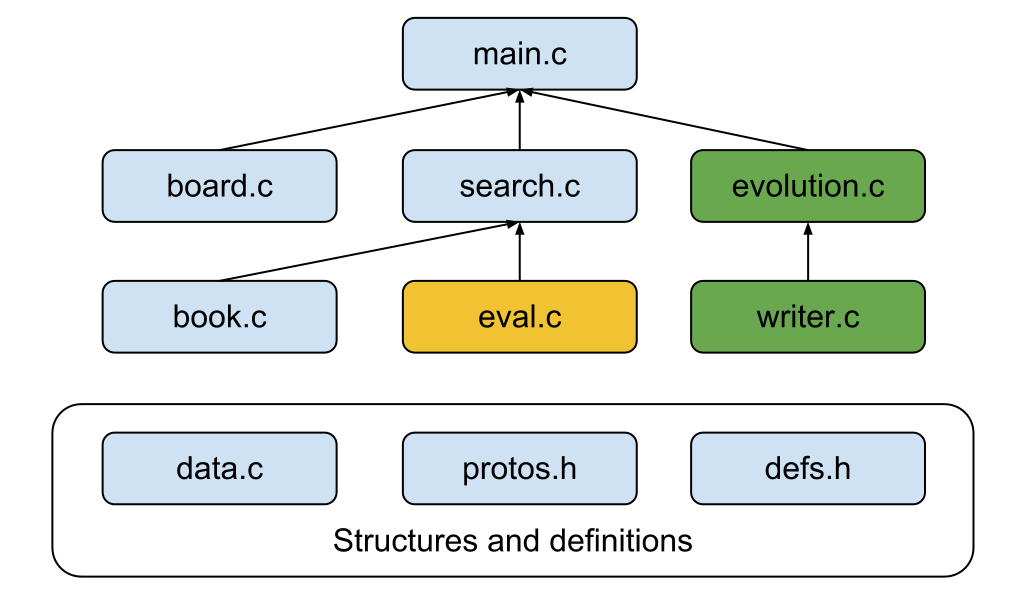
\includegraphics[scale=0.25]{images/Chess_AI_Architecture.png}
\caption{TSCP and evolution algorithm plugin architecture. In green, the evolutionary plugin. In yellow, the evaluation file that is modified to change the values used by the AI.}
\end{figure}
\end{center}

Basically, main.c still controls the flow of the program, but instead of asking for a move to the player, it will ask the evolution.c module for the next game to play by a call to next\_game() method. The writer module takes care of keeping an history file with the best individuals from each generation. It helps with drawing the pieces values charts that we focus on in the results section.

\subsection{Algorithm}
Evolving the values used for the 5 types of pieces that we are interested in is done using an special kind of evolutionary algorithm. We call 'individual' for that algorithm the set of 5 values for pawn, knight, bishop, rook and queen (initial values of respectively 100, 300, 300, 500, 900).

\subsubsection{Evolution strategy}
Before we get into details, it is crucial to understand that the values we are evolving remain the same during a game between two individuals (the BOARD evaluation function uses the same values from the individuals during the same game). Our OWN evaluation function is based on the games that individuals play against each other (with their values feeded into the chess AI for the BOARD evaluation function).\\
The algorithm is described below:
\begin{itemize}
\item The $\mu$ parents breed $\lambda$ children,
\item Children are mutated randomly,
\item Parents and children each play two games against one another (once as black, once as white),
\item Depending on the number of points collected, the $\mu$ better individuals are selected as the new parents for the next generation.
\end{itemize}
The points distributed after one game are as follow:
\begin{itemize}
\item Victory: 3 points,
\item Defeat: 0 point,
\item Stalemate, draw (by repetition or maximum number of moves (50) reached): 1 point.
\end{itemize}
Hence, our evaluation function is relative to the individuals that are part of the generation. However, as we always select the best individuals between parents and children ($\mu + \lambda$ strategy), our approach does not suffer from degeneration of individuals because of the relative evaluation function.

\subsubsection{Boundary checking parameters}
For reasons of convenience, we decided to implement a boundary checking mechanism to ensure that the values remain reasonable throughout the evolution. That prevented some values to get ridiculously far away from their expected range. The ranges that were used are described below:
\begin{itemize}
\item Pawn: 10 < value < 200,
\item Knight: 200 < value < 400,
\item Bishop: 200 < value < 400,
\item Rook: 400 < value < 600,
\item Queen: 700 < value < 1100.
\end{itemize}

\subsubsection{Strategy parameters}
Initially, the random change that was applied to each child was set to be a random integer betweem -15 and 15.

\section{Results and discussion}
We fist describe the experimental parameters before coming to the results (by interpreting the graphs given by the evolution of individuals.

\subsection{Experimental parameters}
\subsection{Evoluted AI}
\subsection{Visual evolution}
\subsection{Conclusion}

\section*{References}


\end{document}

